%\subsection{Safety Verification}

% \begin{figure}
% \centering
% \subfigure[]{%
% 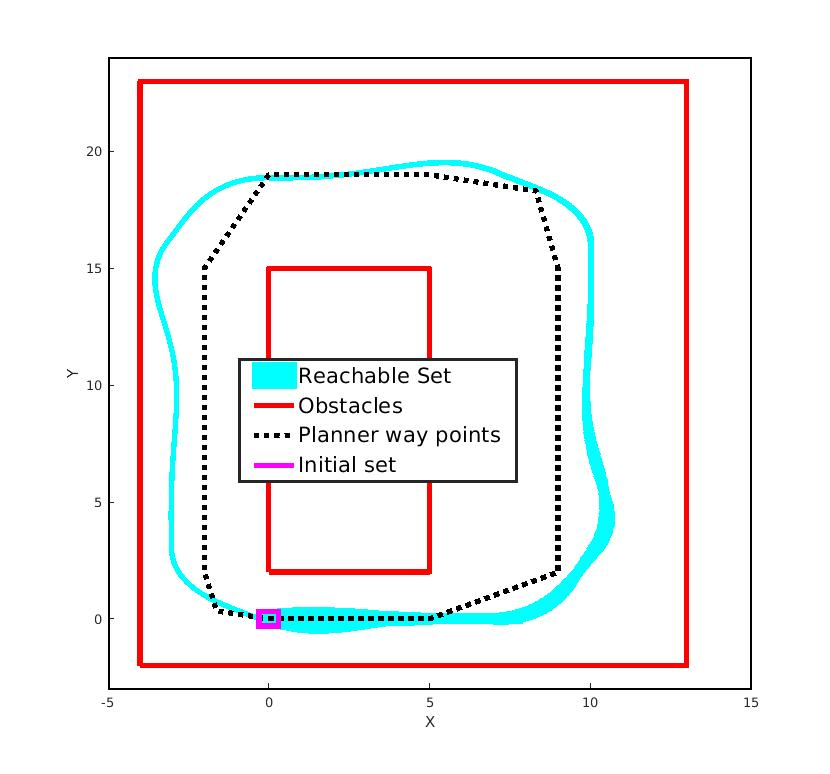
\includegraphics[width=2.65in]{Figures/tracks/track1-voronoi-cora.jpg}%
% \label{fig:track1_voronoi-cora}%
% }\qquad
% \subfigure[]{%
% \includegraphics[width=2.65in]{Figures/tracks/track1-cora.jpg}%
% \label{fig:track1_cora}%
% }
% \caption{Verification with respect to the rectangular track. Each turn depicts a different transition based on the track width. (a) highlights the Voronoi diagram for the track while (b) provides its corresponding reachable set computed in CORA. Different colors in the reachable set are representatives of different locations in the hybrid system model.}
% \label{fig:eval_track1}
% \end{figure}

\begin{figure*}
    \centering
    \subfigure[for small initial set]{\label{fig:track1_voronoi-cora}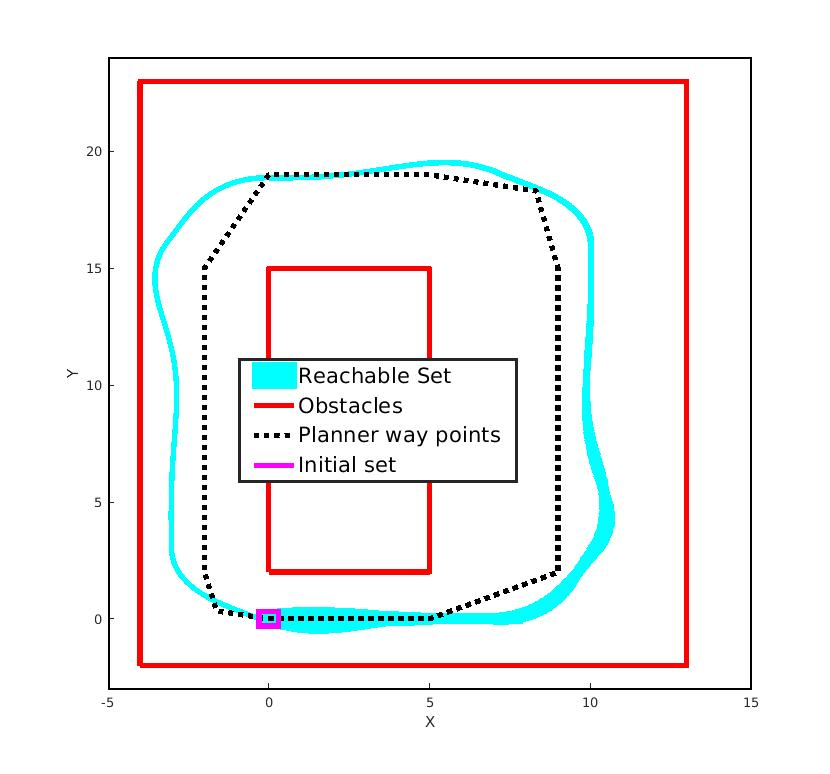
\includegraphics[width=3.2in]{Figures/tracks/track1-voronoi-cora.jpg}}
    \subfigure[for a large initial  set]{\label{fig:track1_cora-abstraction}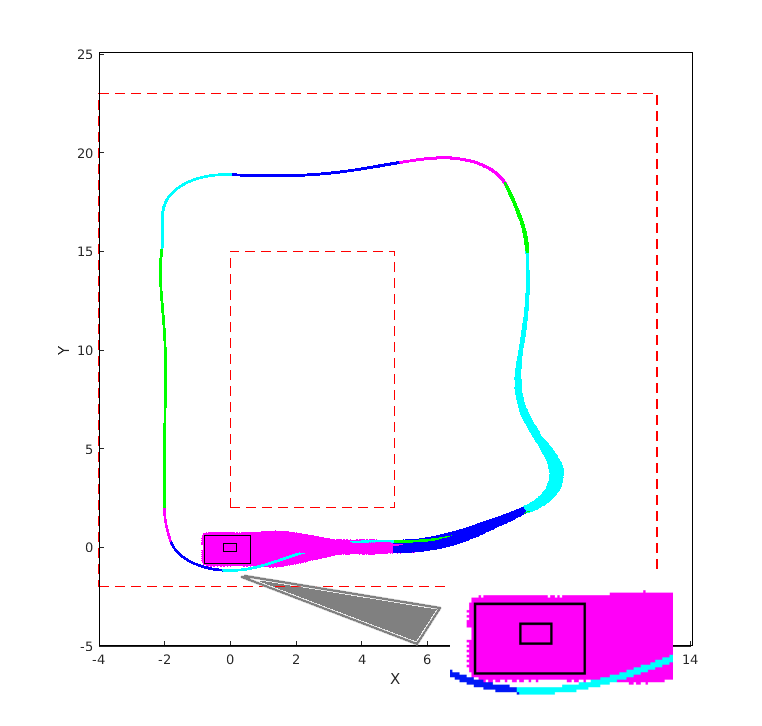
\includegraphics[width=3.2in]{Figures/tracks/reachMap-obstacle_zoomed.png}}
    \caption{\textbf{Reachable set computation for Track-1}. In Fig.~\ref{fig:track1_voronoi-cora}, the fixed point is obtained in mode 3 in the second lap. The filled black rectangle depicts the initial set. In Fig.~\ref{fig:track1_cora-abstraction}, the smaller rectangle corresponds to the fixed point partition and larger one is the originally given initial set.}
\label{fig:eval_track1}
\end{figure*}

% \begin{figure}
% \centering
% \subfigure[]{%
% 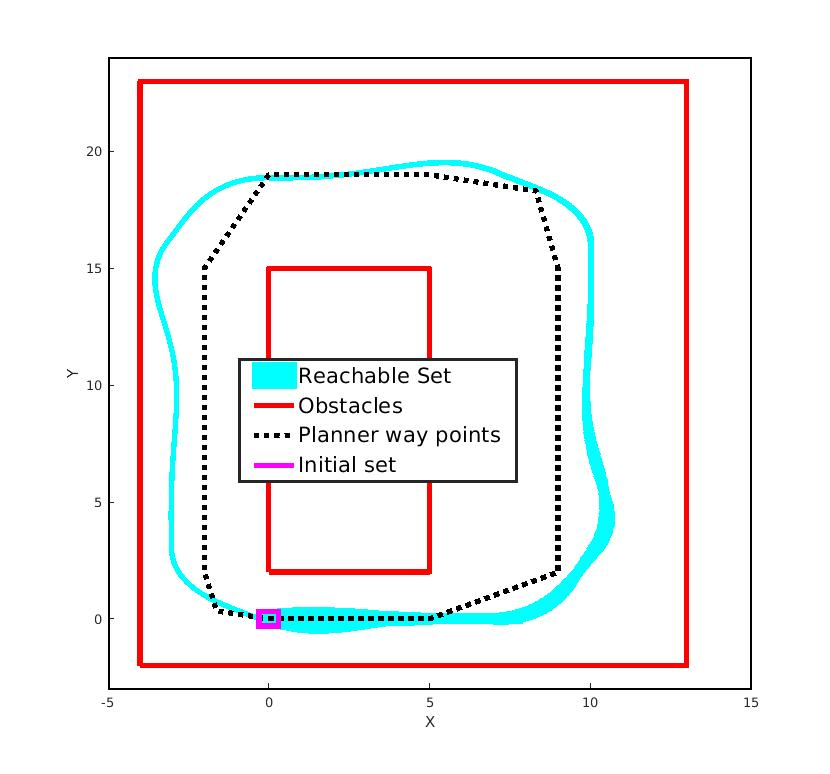
\includegraphics[width=\linewidth]{Figures/tracks/track1-voronoi-cora.jpg}%
% \label{fig:track1_voronoi-cora}%
% }\qquad
% \subfigure[]{%
% 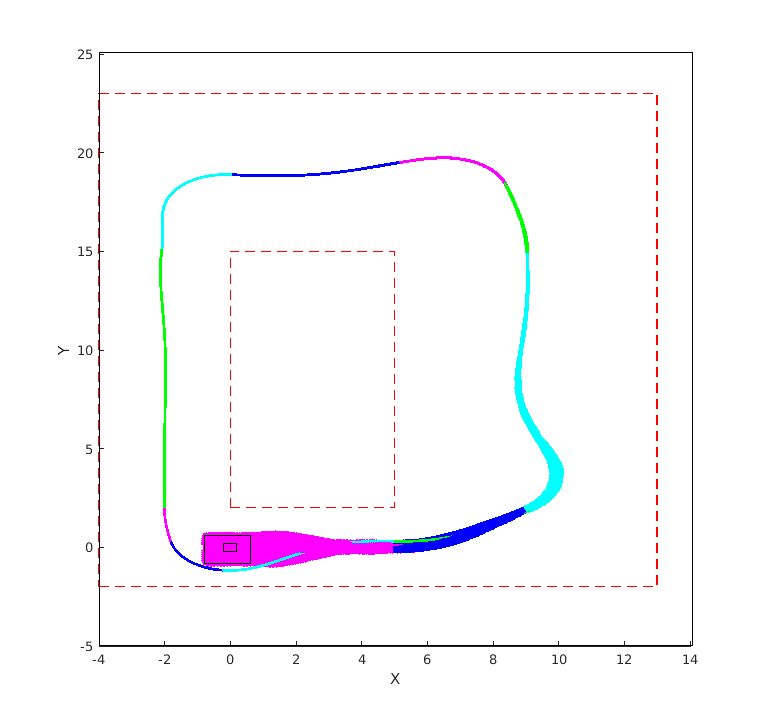
\includegraphics[width=3.4in]{Figures/tracks/reachMap-obstacle.png}%
% \label{fig:track1_cora-abstraction}%
% }
% \caption{Verification with respect to the rectangular track. Each turn depicts a different transition based on the track width. (a) highlights the Voronoi diagram for the track while (b) provides its corresponding reachable set computed in CORA. Different colors in the reachable set are representatives of different locations in the hybrid system model.}
% \label{fig:eval_track1}
% \end{figure}

We experiment with multiple safety verification platforms such as CORA~\cite{Althoff2018b}, Flow*~\cite{10.1007/978-3-642-39799-8_18}, and C2E2~\cite{Duggirala.2015} for non-linear hybrid systems. Different platforms use different symbolic representations for the reachable set. For instance, Flow* uses Taylor models, C2E2 uses Jacobian matrix and discrepancy functions, and CORA primarily makes use of zonotopes for representing the reachable sets. As their utility is application specific,  we observed that overapproximation error in both C2E2 and Flow* is very high for our case studies. One possible reason could be that Taylor model approximation in Flow* and discrepancy function computed in C2E2 are too conservative. We illustrate the  reachable set accuracy across Flow* and CORA on a small system in Section~\ref{subsec:appendix-reach-set-accuracy} in the Appendix.

% Our efforts with another simulation based  verification tool, DryVR~\cite{Qi.2018}, 

%Suppose the track is defined in a stationary $(x, y)$ frame, $\theta$ is the vehicle's orientation and 
%$\ell$ is the look ahead distance. 

%
% Fig.~\ref{fig:sim1_flow} represents the car's trajectory starting from a particular initial configuration, as computed in Flow*. 

%%%%% Sridhar: the below segment is already in appendix. Removing it.
% As a part of experimentation, we perform the reachable set computation in Flow* and CORA by modeling a single turn on the track as the hybrid automata. 
% %
% The initial set is given as intervals over state variables i.e., $x \in [0.0, 0.5]$, $y \in [0.9, 1.1]$ and $\theta \in [-0.5, -0.5]$. 
% %
% The reachable sets computed in both tools are shown in figures~\ref{fig:reachSet1_flow} and~\ref{fig:reachSet1_cora}. 
% %
% The divergent behavior of the reachable set in Flow* is seemingly due to error compounded over time because of coarse approximation. 
% %
% The figures also illustrate that the vehicle while turning swings to some extent before merging back on to the track.

In the safety verification of our dynamical model, the obstacles or walls constitute the unsafe set i.e., the objective is to verify that the reachable set does not overlap with the walls. 
%
% For each track given as the polygonal walls, we obtain the global Voronoi diagram, linearize the curved edges resulting into a piece-wise linear Voronoi edges. 
%
% The given sequence of Voronoi edges is modeled as the hybrid automata. Typically, a hybrid automata has as many discrete modes as the number of Voronoi edges. 
The initial set considered during reachable set computation in track-1 is $x \in [-0.3, 0.3]$, $y \in [-0.3, 0.3]$ and $\theta \in [-0.2, 0.2]$.
The Voronoi diagram and the corresponding reachable set for track-1 are shown in Fig.~\ref{fig:track1_voronoi-cora}. Based on the track width, the turns in this track encompass 4 different transitions - wide to narrow, wide to wide, narrow to narrow, and narrow to wide. 
%
Also observe that the fixed point of the reachable set computation is obtained in \emph{mode 3} in lap 2. The values of state variables in \emph{mode 3} across lap-1 and lap-2 are depicted in Fig.~\ref{fig:track1-fixed-point-loc3} that establishes our fixed point claim. The reachable set computation results for other tracks are illustrated in Fig.~\ref{fig:eval_track2-track3-track4-track5} in the Appendix. CORA takes roughly a minute to compute the reachable set for each track.
%, which is considered fast in the verification domain.

% Fig.~\ref{fig:eval_track2} depicts the results obtained for more generalized track. It respectively takes 16 sec and 23 sec to verify the model for  rectangular and general tracks. Note that in both scenarios, after completing first lap, the reachable set achieves a fixed point during second location.

%
% Also, the overapproximation of the reachable set increases when the vehicle switches from one line segment to the next (potentially because of overapproximating the guard set). 
%
An observation from the safety verification results is that if the set of initial conditions is large (larger uncertainty of vehicle's initial orientation and position with respect to the map), CORA fails to compute the reachable set over-approximation. 
%
As suggested earlier, this can potentially be mitigated by fixed-point based partitioning of the large initial set and verifying the safety for each partition.

We have implemented the automatic partitioning algorithm and evaluated the approach on track-1 for the initial set $x \in [-0.8, 0.6]$, $y \in [-0.8, 0.6]$ and $\theta \in [-0.2, 0.2]$. CORA fails to compute the reachable set for this initial set. 
%
Our technique keeps partitioning the set until it finds a  partition $x \in [-0.2, 0.2]$, $y \in [-0.2, 0.2]$ and $\theta \in [-0.2, 0.2]$ having a fixed point. (We do not partition $\theta$ in this case).
%
Once the fixed point is found, the rest of the initial set is partitioned into intervals of the given width and reachable set is computed for each partition. In addition, at each step, reachable set containment w.r.t. the fixed point is conducted to avoid redundant computation. Fig.~\ref{fig:track1_cora-abstraction} demonstrates the safe reachable set successfully computed by our approach  for the given set.


We also performed reachable set computation using CORA over tracks where the vehicle had to take a steep turn (turns of more than 90 degrees). For such instances, CORA failed to compute an overapproximation of the reachable set that is sufficient to establish the safety even for small initial sets. This shows that there is room for improvement in the current reachable set computation methods.

%The second set of figures ~\ref{fig:reachSet2_flow} and ~\ref{fig:reachSet2_cora} depicts the set of reachable states for the initial set $x \in [0.0, 0.0]$, $y \in [0.0, 0.0]$ and $\theta \in [-0.2, 0.2]$.
% \begin{figure}
% \centering
% \subfigure[]{%
% 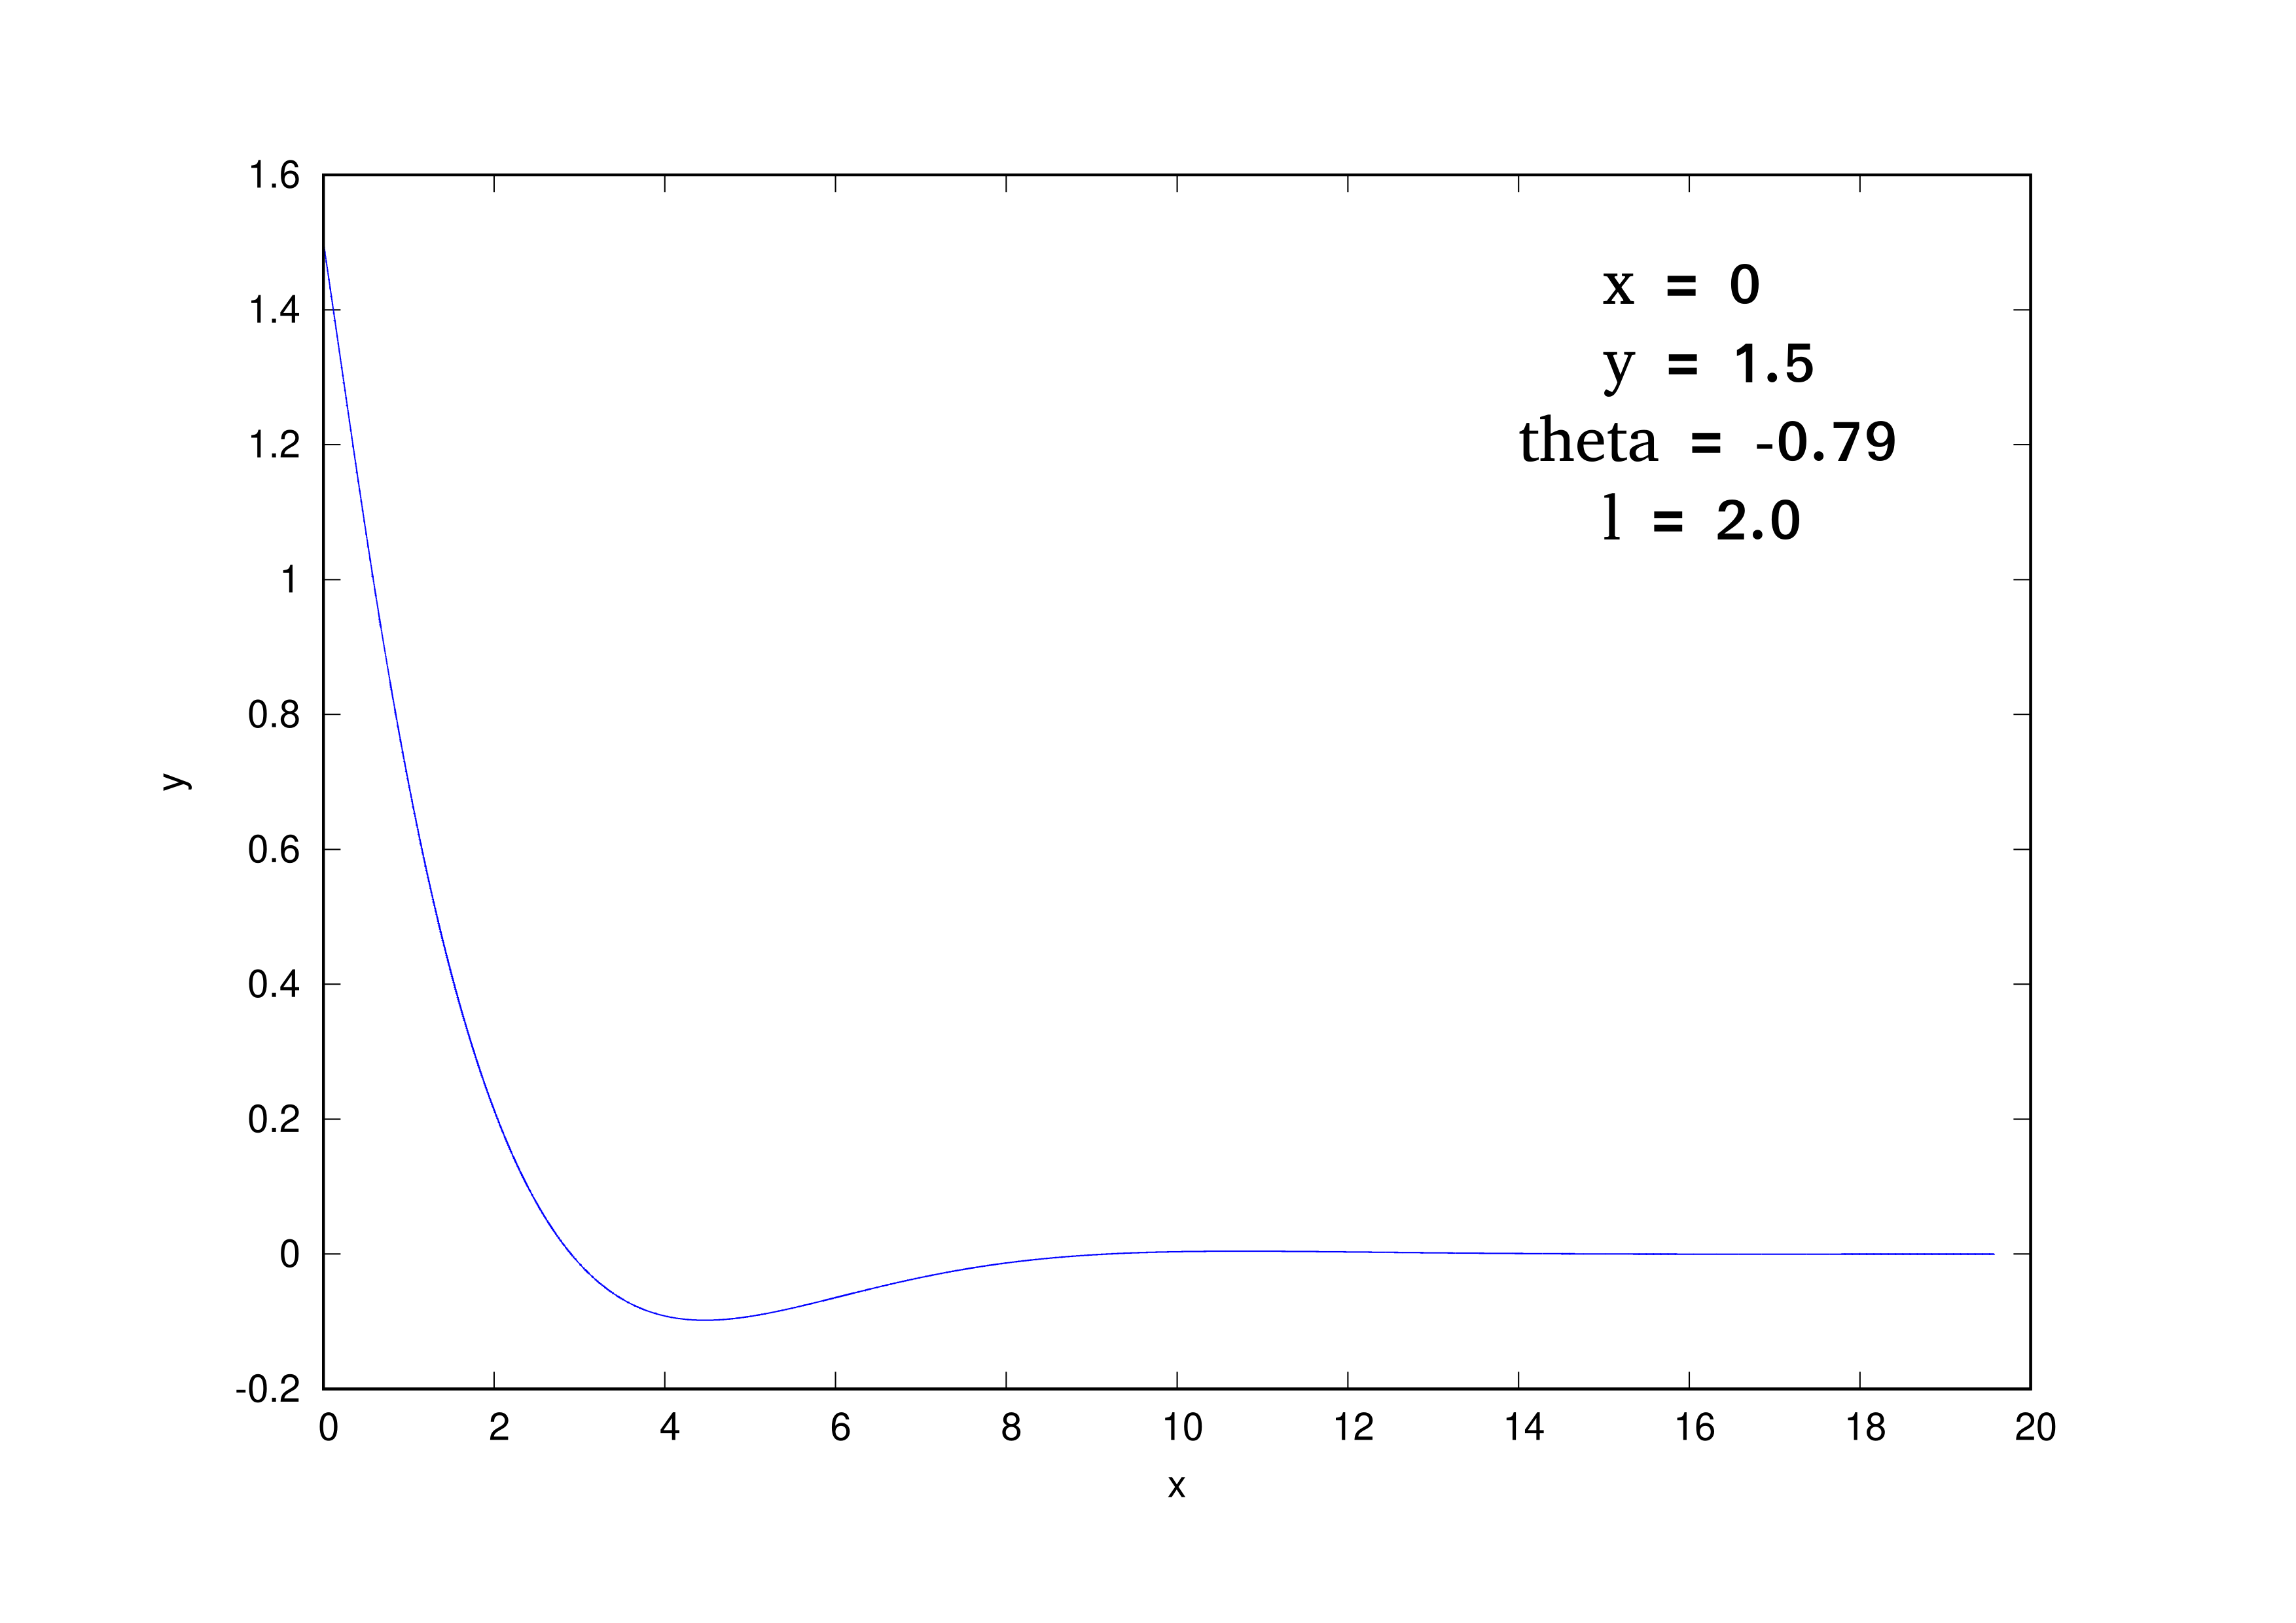
\includegraphics[width=2.8in]{Figures/flow_pure_pursuit_1.png}%
% \label{fig:traj1_flow}%
% }\qquad
% \subfigure[]{%
% 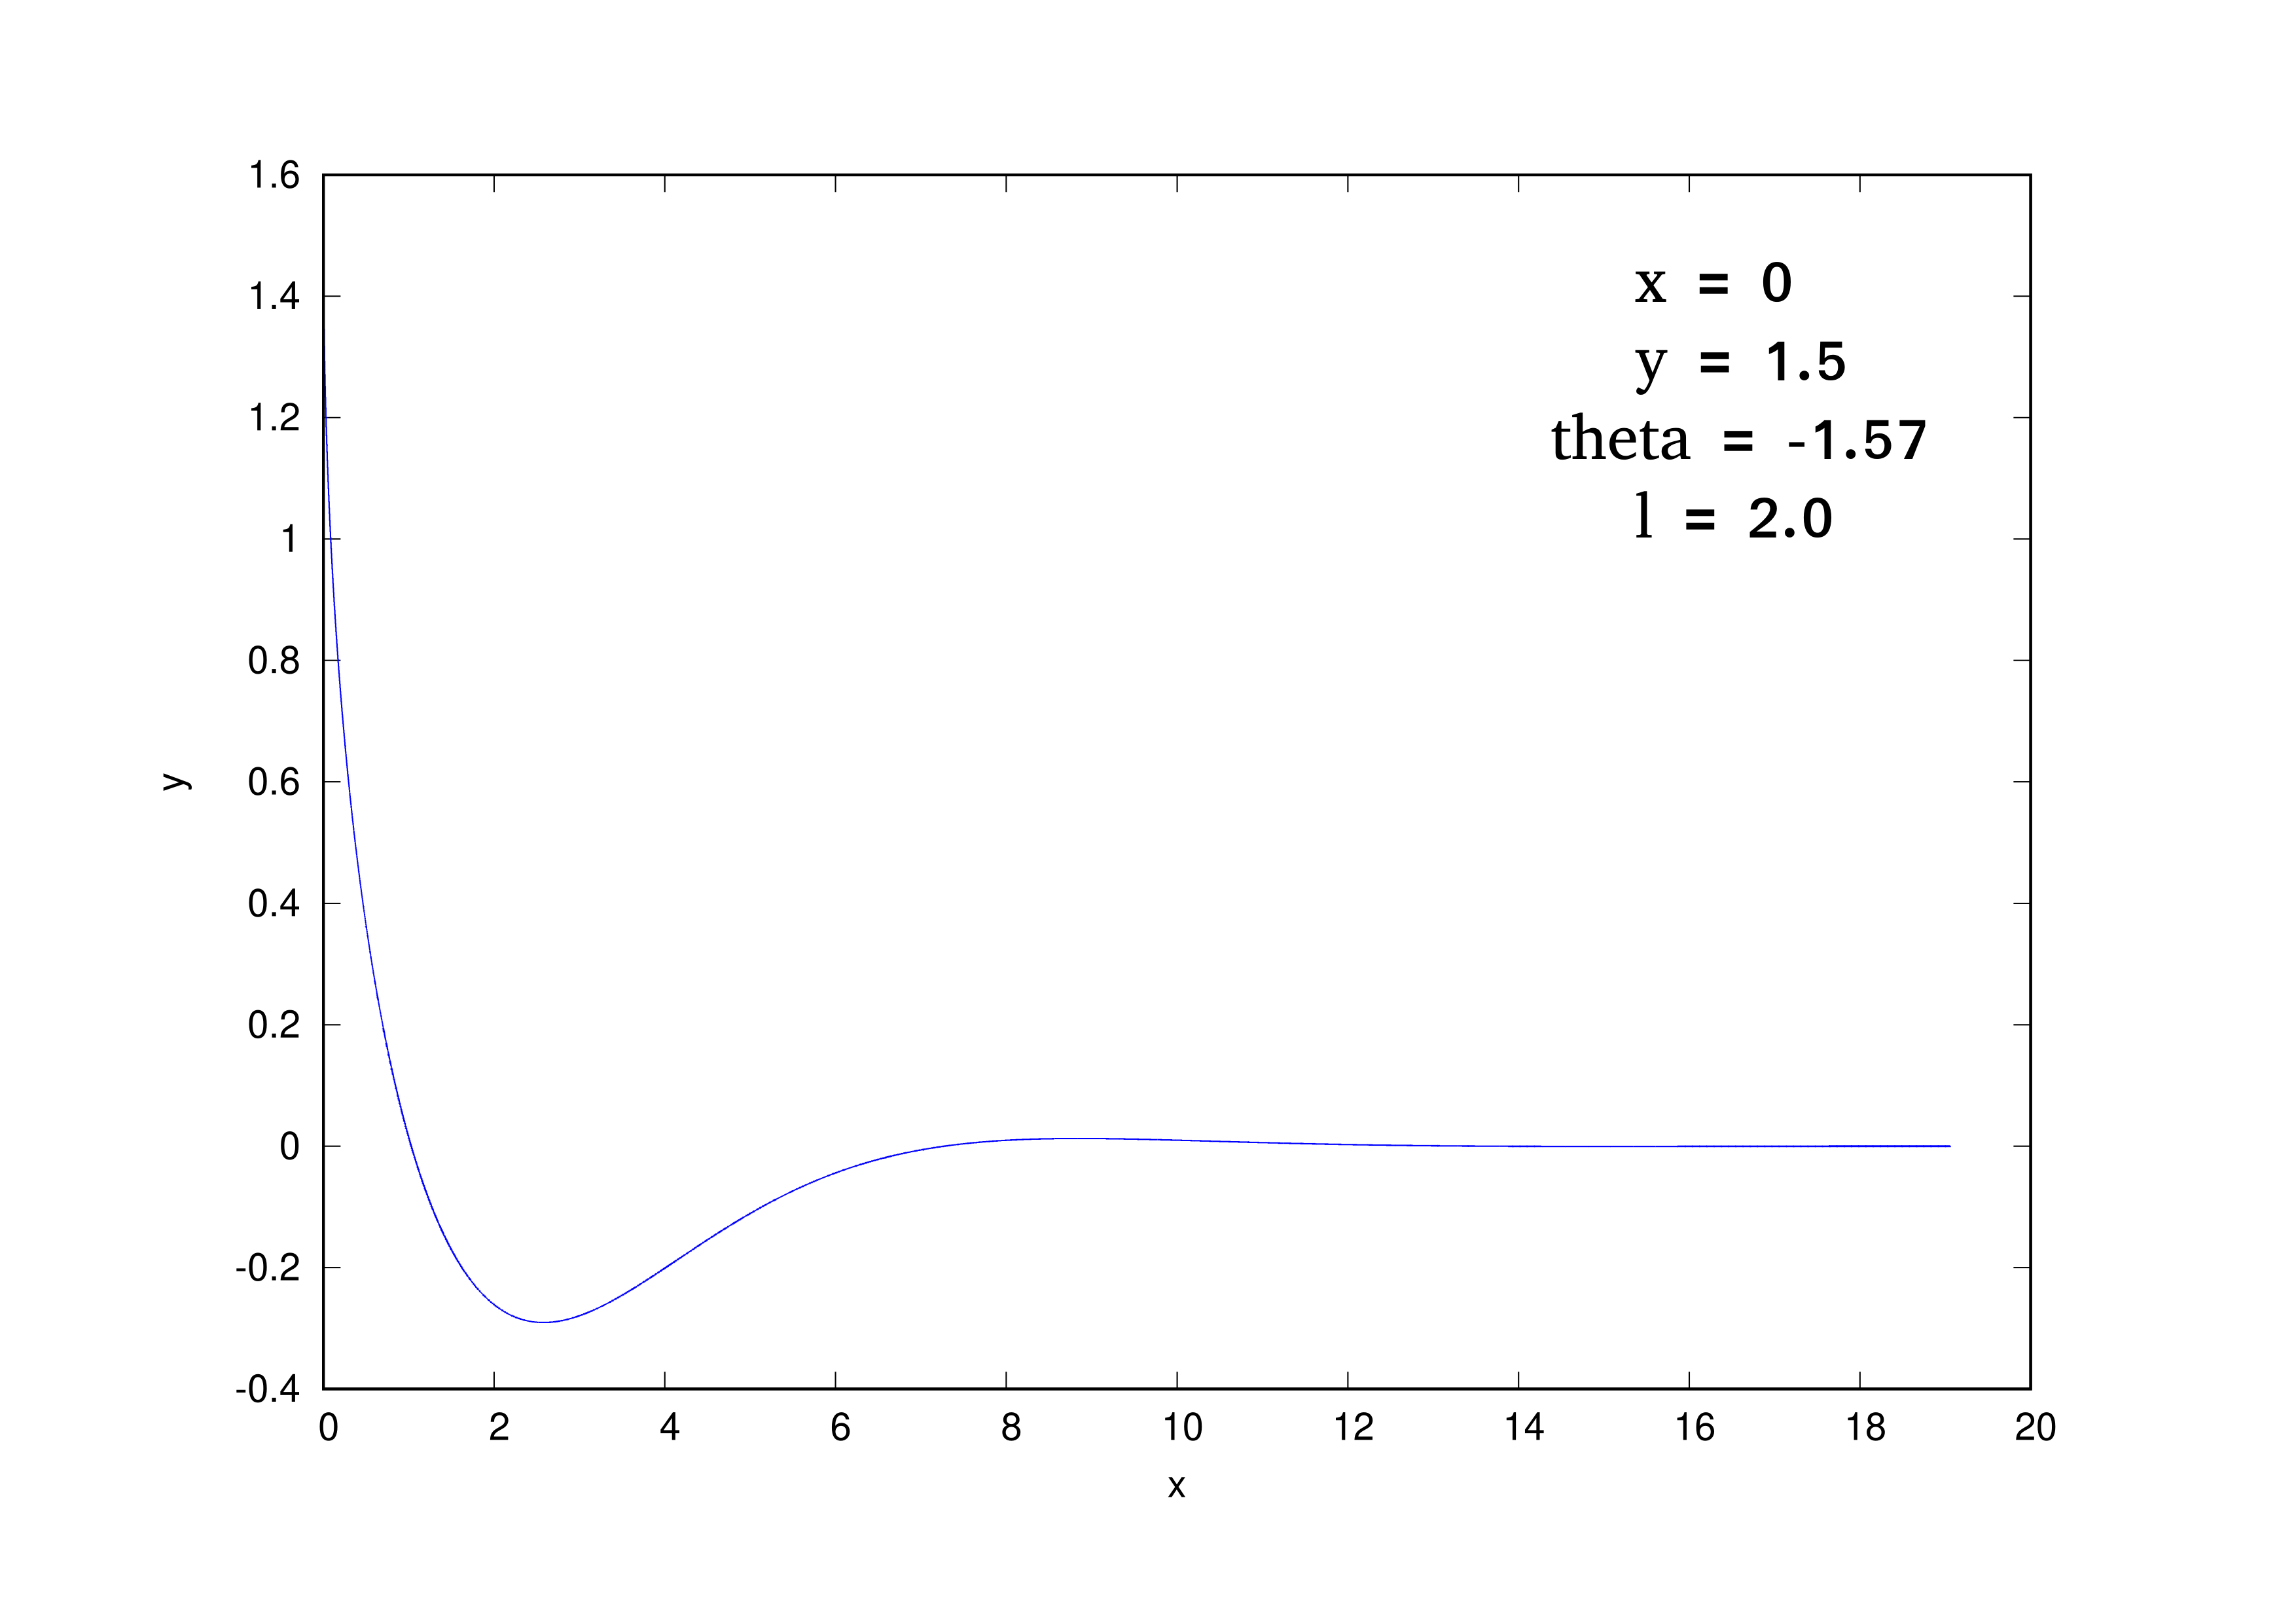
\includegraphics[width=2.8in]{Figures/flow_pure_pursuit_2.png}%
% \label{fig:traj2_flow}%
% }
% \subfigure[]{%
% 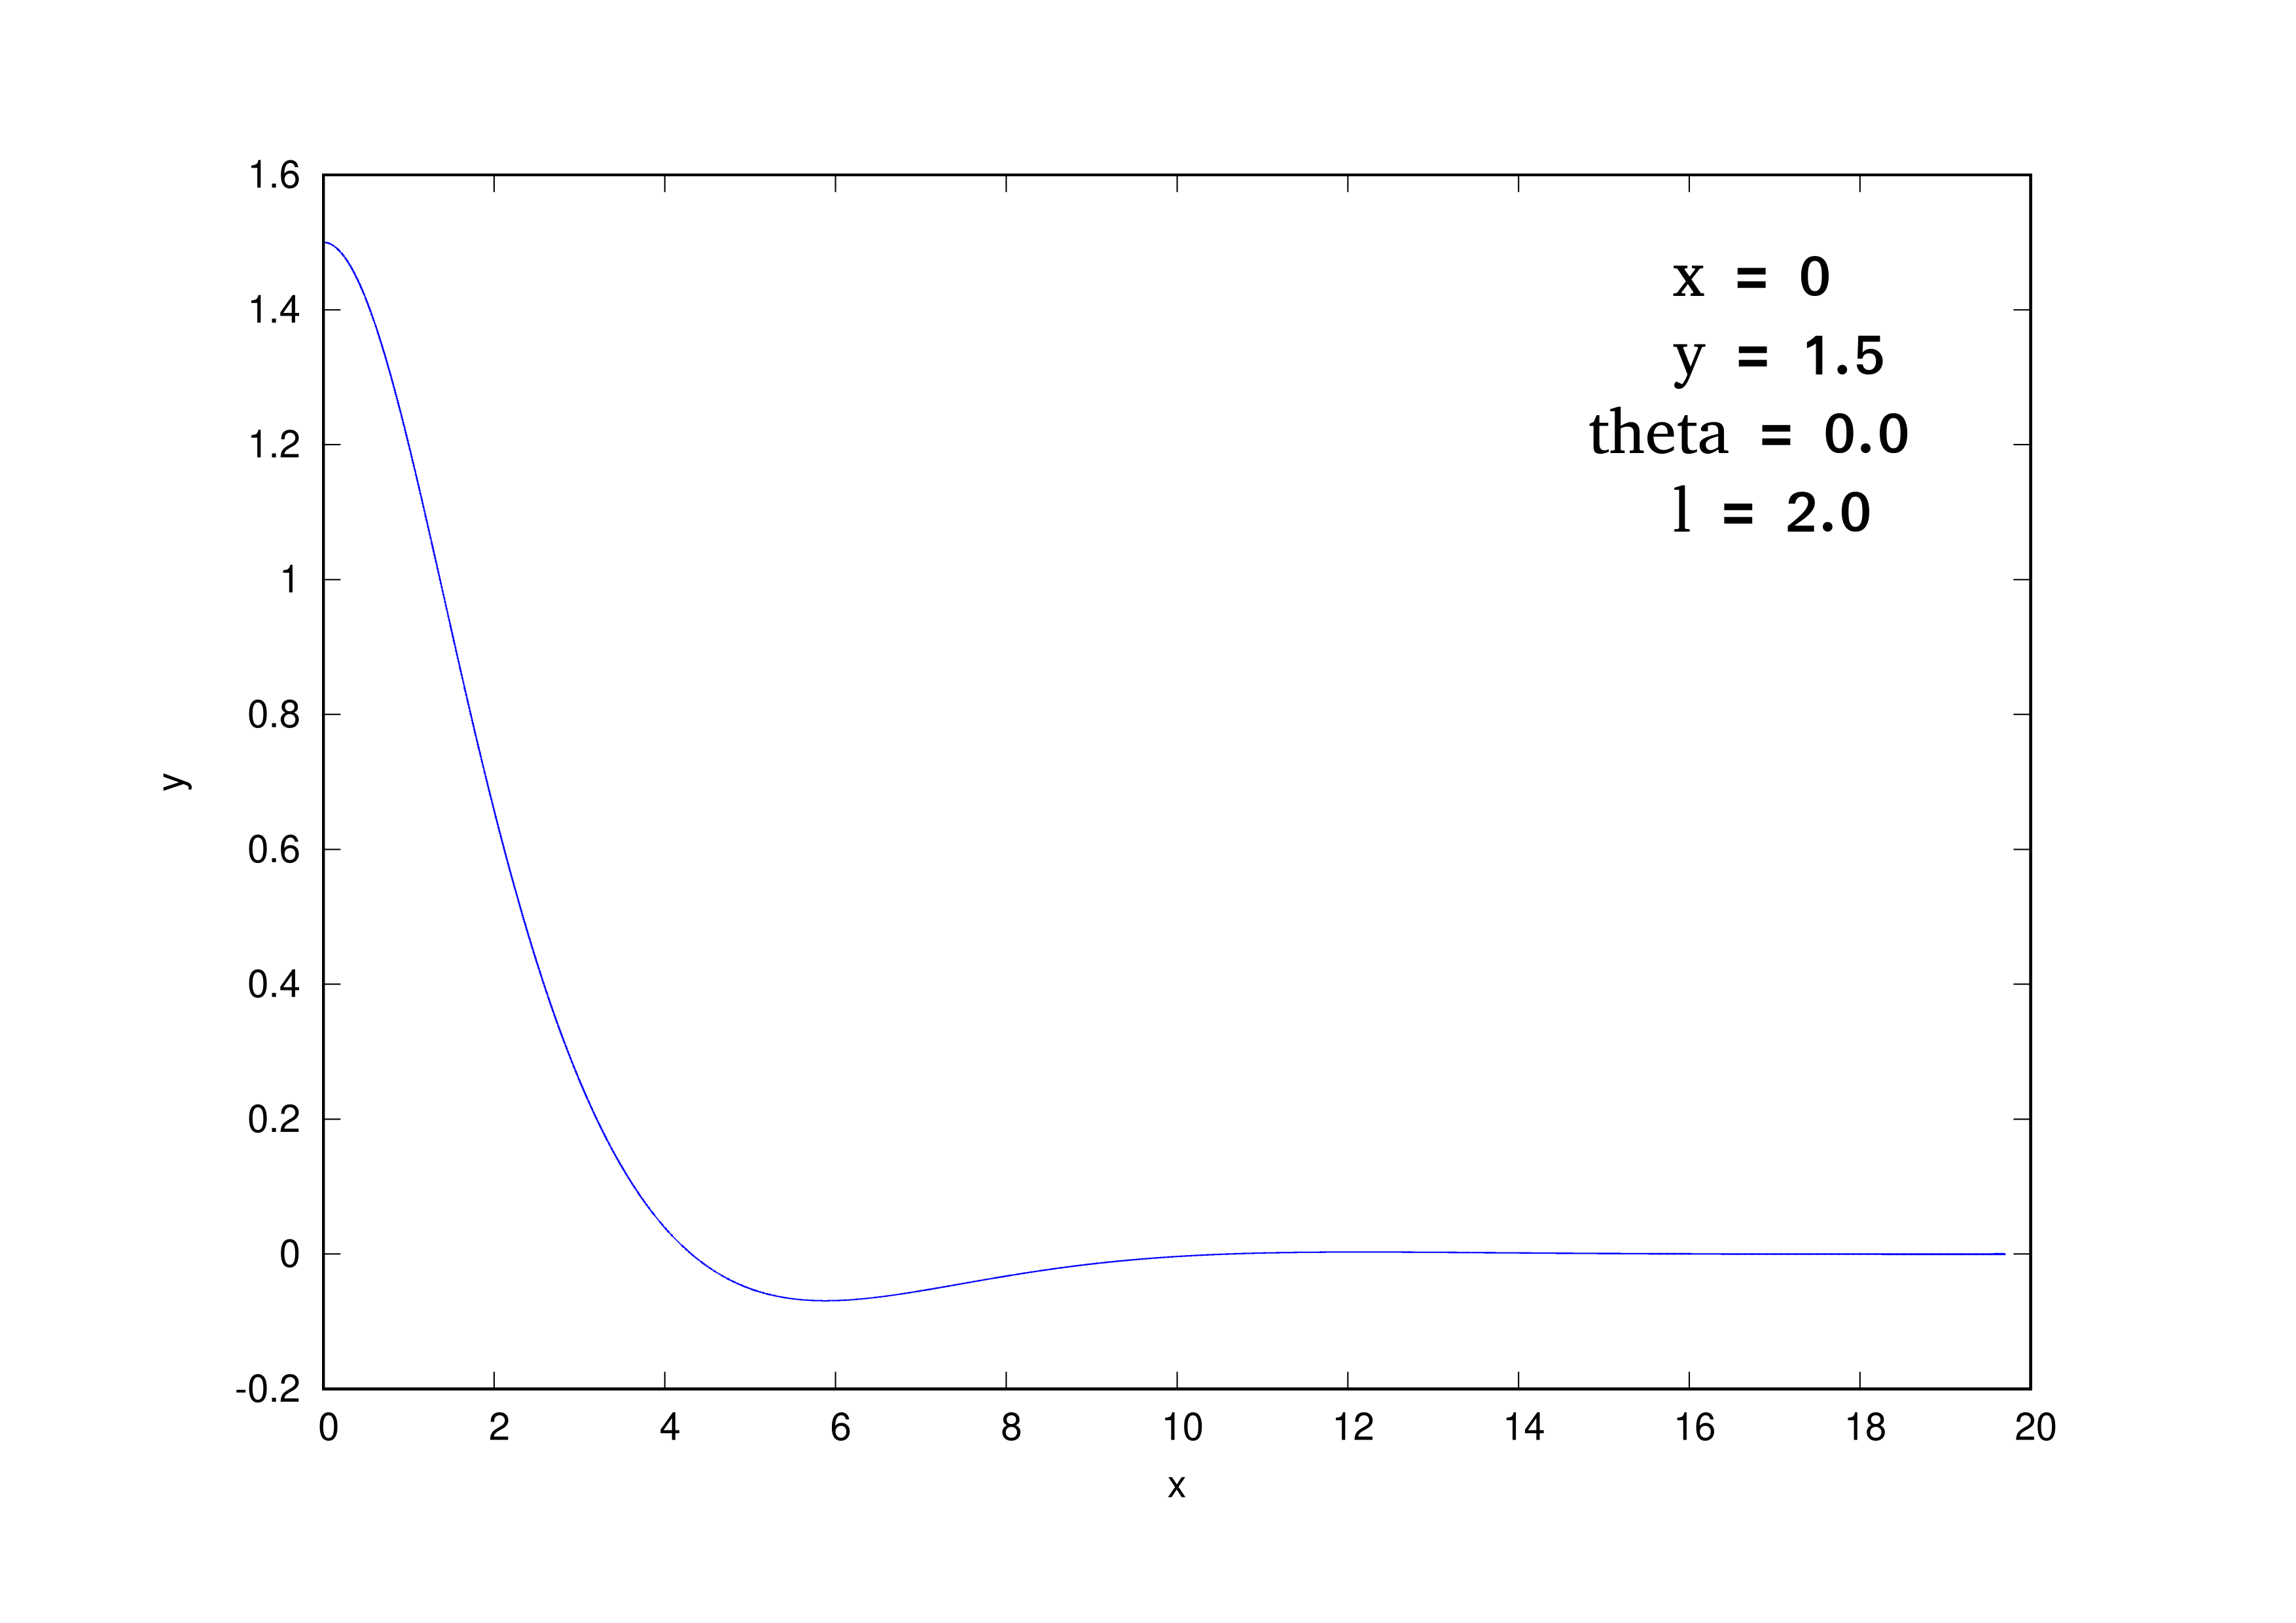
\includegraphics[width=2.8in]{Figures/flow_pure_pursuit_3.png}%
% \label{fig:traj3_flow}%
% }\qquad
% \subfigure[]{%
% 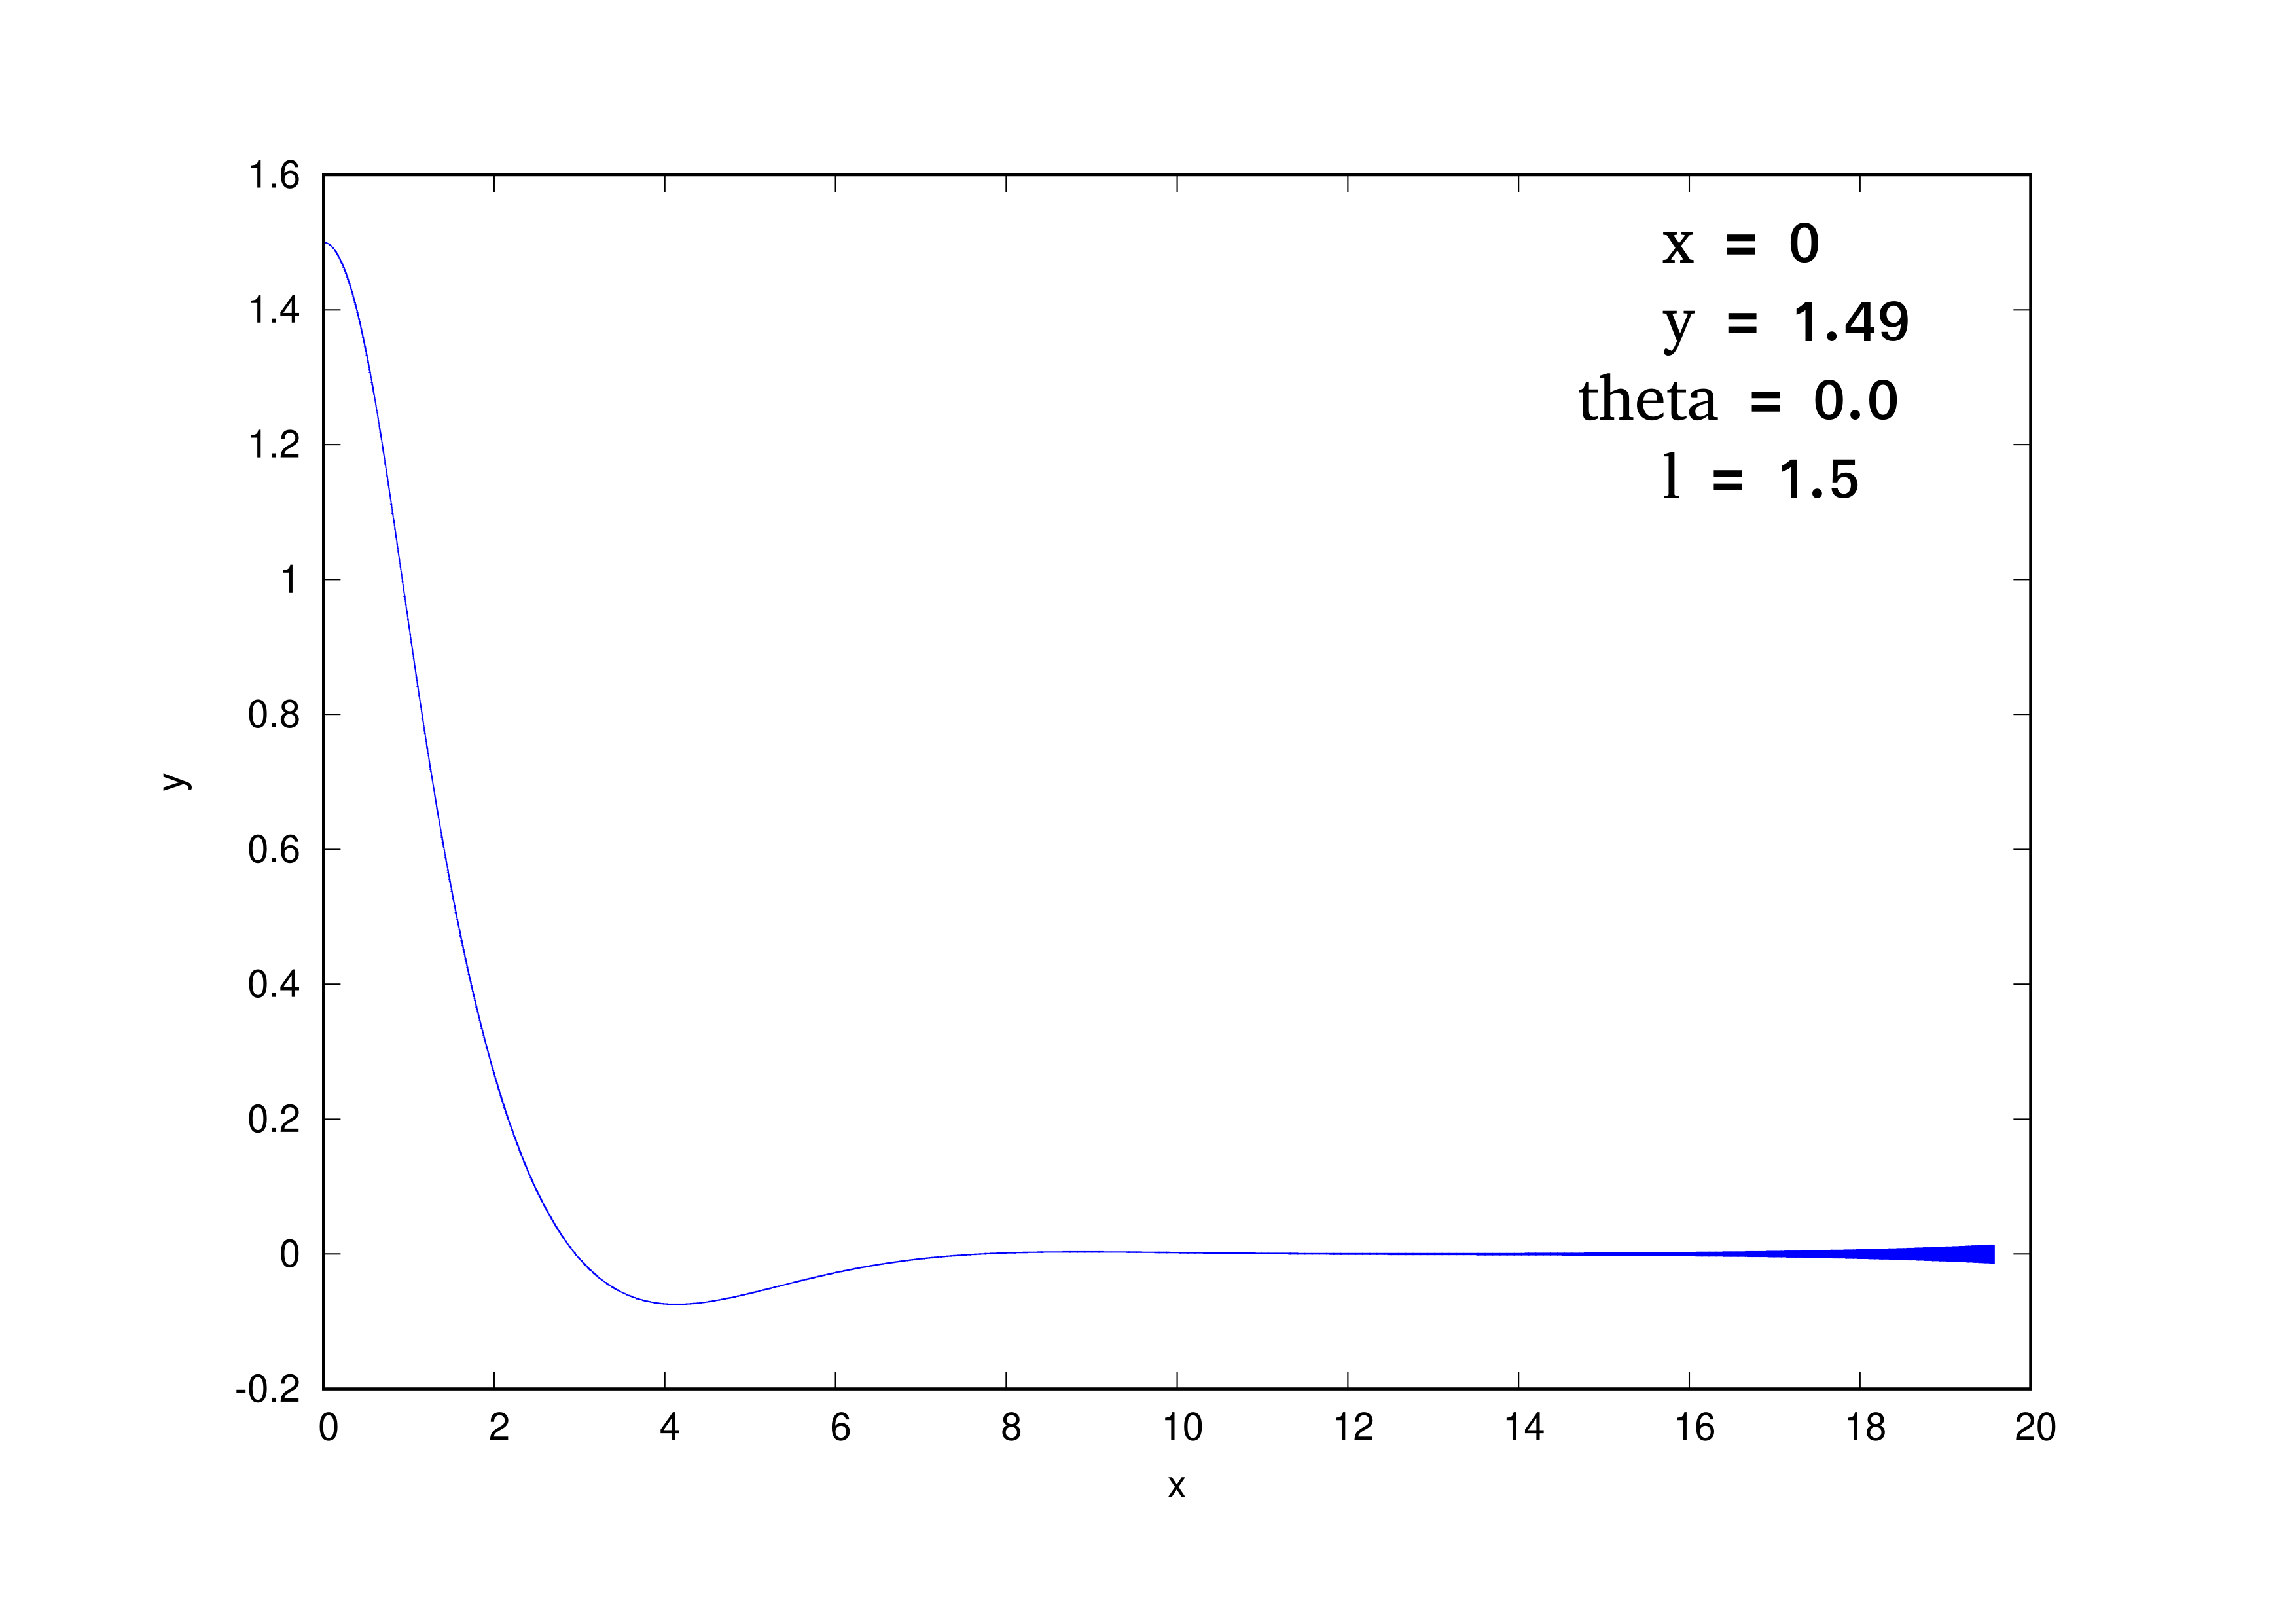
\includegraphics[width=2.8in]{Figures/flow_pure_pursuit_4.png}%
% \label{fig:traj4_flow}%
% }
% \caption{Vehicle trajectories computed using Flow*. The time step and time bound for simulations are 0.001 sec and 20 sec respectively.}
% \label{fig:traj_flowstar}
% \end{figure}


